\documentclass[11pt,a4paper,landscape]{article}

% ============================================================
% PACKAGES & SETUP
% ============================================================
\usepackage[utf8]{inputenc}
\usepackage[T1]{fontenc}
\usepackage{helvet}
\renewcommand{\familydefault}{\sfdefault}

\usepackage{amssymb}
\usepackage{xcolor}
\usepackage[top=1.0cm,bottom=1.2cm,left=1.2cm,right=1.2cm,footskip=16pt]{geometry}
\usepackage{tikz}
\usetikzlibrary{calc,positioning,fit}
\usepackage{hyperref}
\usepackage{fancyhdr}
\usepackage{enumitem}

% ============================================================
% COLOR PALETTE (Dark Navy / Charcoal / Minimal Accent)
% ============================================================
\definecolor{NavyBlue}{RGB}{15,23,42}       % Primary headers / title
\definecolor{DarkSlate}{RGB}{30,41,59}      % Body text
\definecolor{SteelGrey}{RGB}{71,85,105}     % Subtitles & borders
\definecolor{LightBg}{RGB}{248,250,252}     % Card background
\definecolor{BorderColor}{RGB}{226,232,240} % Card borders
\definecolor{TealAccent}{RGB}{14,116,144}   % Minimal accent

% ============================================================
% PDF METADATA
% ============================================================
\hypersetup{
    colorlinks=true,
    linkcolor=NavyBlue,
    citecolor=NavyBlue,
    urlcolor=TealAccent,
    pdftitle={MetaRadar — 4-Week Prototype Development Timeline},
    pdfauthor={Aura Pharmers}
}

% ============================================================
% HEADER / FOOTER
% ============================================================
\pagestyle{fancy}
\fancyhf{}
\renewcommand{\headrulewidth}{0pt}
\renewcommand{\footrulewidth}{0.5pt}
\renewcommand{\footrule}{\color{BorderColor}\hrule width\headwidth height 0.5pt \vspace{3pt}}

\fancyfoot[L]{%
    \small\color{SteelGrey}
    Illustrative 4-week prototype roadmap --- scope and sequencing may evolve during implementation.
}
\fancyfoot[R]{%
    \small\color{SteelGrey}\textbf{MetaRadar v5.1} --- Technical Development Plan
}

\setlength{\parindent}{0pt}
\setlength{\parskip}{0pt}

\begin{document}

% ============================================================
% DOCUMENT HEADER
% ============================================================
\begin{minipage}[t]{0.70\textwidth}
    {\fontsize{20}{24}\selectfont\bfseries\color{NavyBlue} MetaRadar --- 4-Week Prototype Development Timeline}\\[4pt]
    {\fontsize{10}{13}\selectfont\color{SteelGrey} Technical Implementation Sequence for Near-Real-Time Competitive Intelligence Prototype}
\end{minipage}%
\begin{minipage}[t]{0.30\textwidth}
    \raggedleft
    \vspace*{2pt}
    {\small\color{NavyBlue}\textbf{Target Domain:} Haemophilia / Rare Disease}\\[2pt]
    {\small\color{SteelGrey} Architecture: Next.js 16 + FastAPI + PostgreSQL}
\end{minipage}

\vspace{10pt}
\hrule height 1pt color BorderColor
\vspace{12pt}

% ============================================================
% HORIZONTAL TIMELINE FLOW ARROW
% ============================================================
\begin{center}

\begin{tikzpicture}[x=1cm, y=1cm]
    % Central Progress Line
    \draw[line width=2pt, color=TealAccent!40, ->] (0,0) -- (26.6,0);
    
    % Milestone Nodes along the axis
    \node[circle, fill=TealAccent, inner sep=3pt, label=below:{\scriptsize\color{SteelGrey}\textbf{KICKOFF}}] at (0.2,0) {};
    \node[circle, fill=TealAccent, inner sep=3pt, label=below:{\scriptsize\color{SteelGrey}\textbf{WEEK 1 GATE}}] at (6.8,0) {};
    \node[circle, fill=TealAccent, inner sep=3pt, label=below:{\scriptsize\color{SteelGrey}\textbf{WEEK 2 GATE}}] at (13.4,0) {};
    \node[circle, fill=TealAccent, inner sep=3pt, label=below:{\scriptsize\color{SteelGrey}\textbf{WEEK 3 GATE}}] at (20.0,0) {};
    \node[circle, fill=TealAccent, inner sep=3.5pt, label=below:{\scriptsize\color{TealAccent}\textbf{PROTOTYPE DEMO}}] at (26.2,0) {};
\end{tikzpicture}
\end{center}

\vspace{8pt}

% ============================================================
% 4-WEEK MILESTONE CARDS IN TIKZ
% ============================================================
\begin{center}
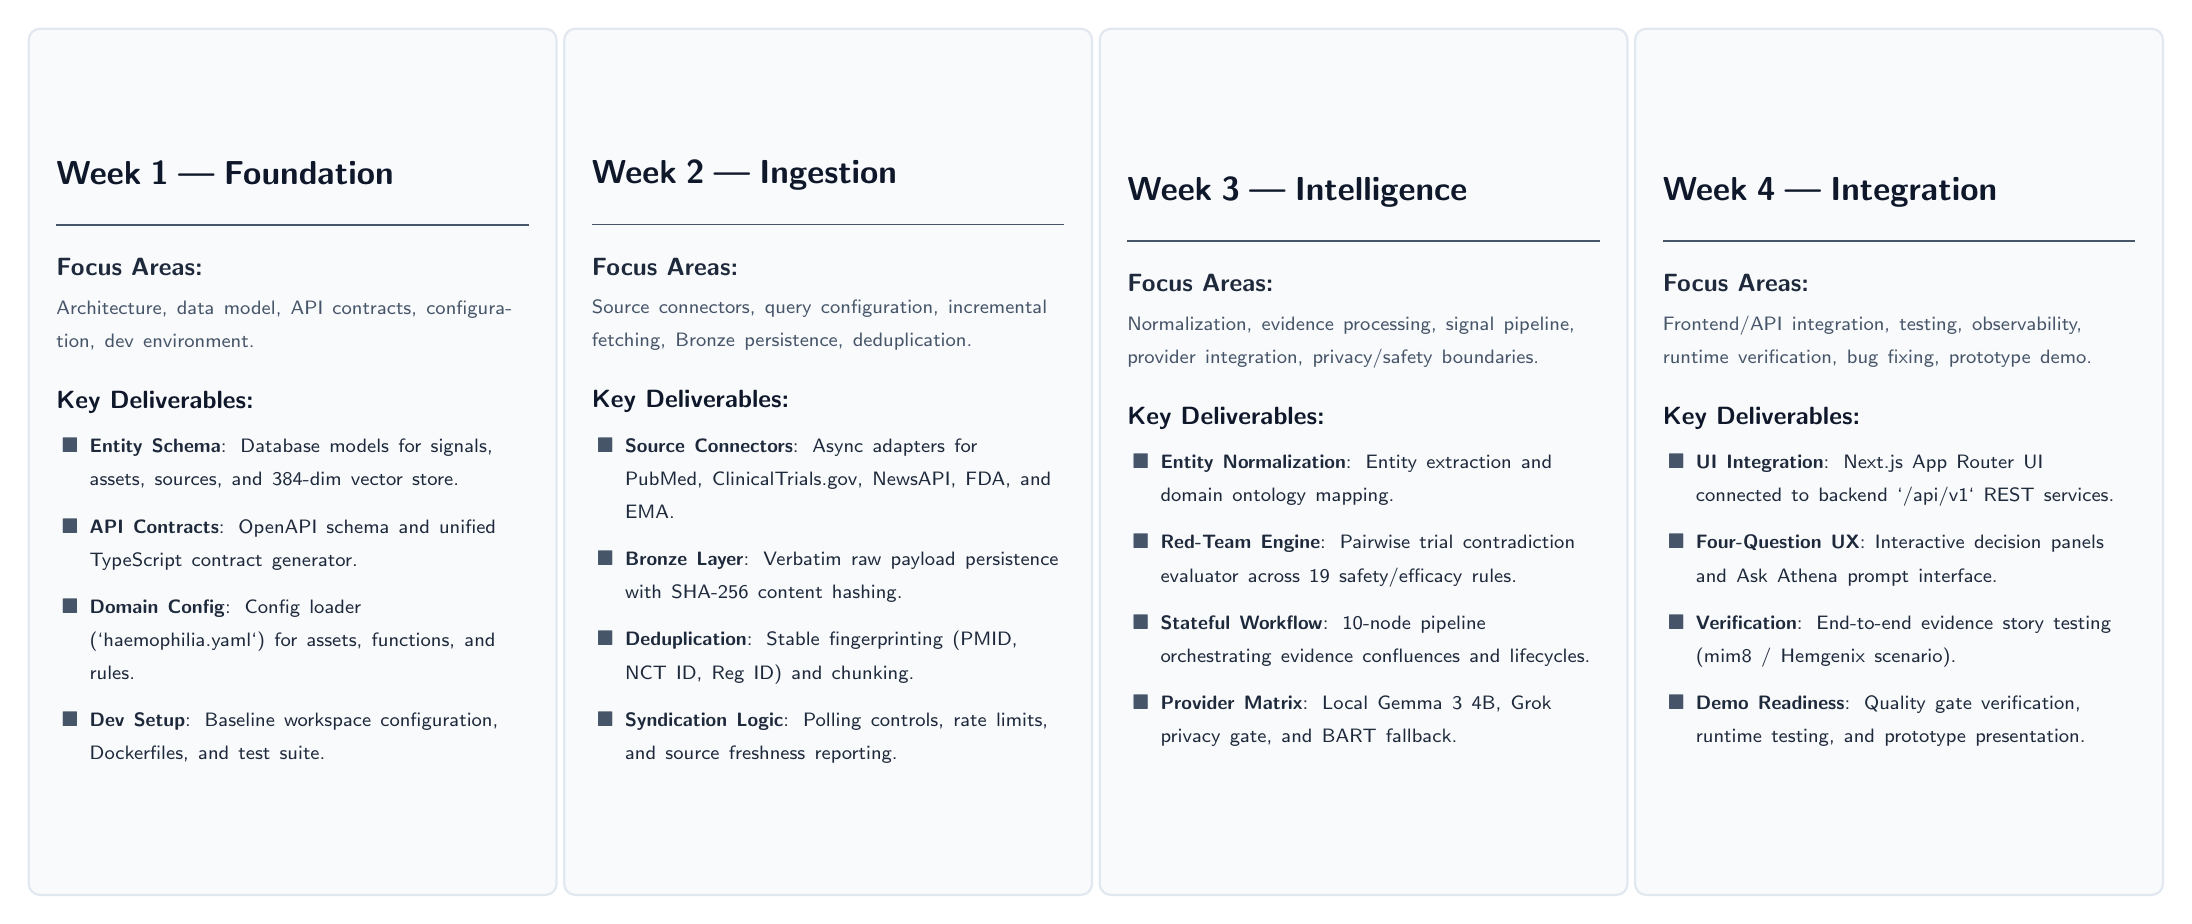
\begin{tikzpicture}[x=1cm, y=1cm]

% ------------------------------------------------------------
% WEEK 1 CARD
% ------------------------------------------------------------
\node[
    draw=BorderColor,
    fill=LightBg,
    rounded corners=4pt,
    line width=0.8pt,
    inner sep=10pt,
    text width=6.0cm,
    minimum height=11.0cm,
    align=left,
    anchor=north west
] (week1) at (0,0) {
    \color{NavyBlue}\textbf{\large Week 1 --- Foundation}\\[3pt]
    \color{SteelGrey}\rule{\linewidth}{0.5pt}\\[6pt]
    {\small\color{DarkSlate}\textbf{Focus Areas:}}\\[2pt]
    {\scriptsize\color{SteelGrey} Architecture, data model, API contracts, configuration, dev environment.}\\[10pt]
    {\small\color{NavyBlue}\textbf{Key Deliverables:}}\\[4pt]
    \begin{itemize}[leftmargin=12pt,labelsep=4pt,itemsep=5pt,parsep=0pt,topsep=0pt]
        \item[\scriptsize$\blacksquare$] {\scriptsize\color{DarkSlate}\textbf{Entity Schema}: Database models for signals, assets, sources, and 384-dim vector store.}
        \item[\scriptsize$\blacksquare$] {\scriptsize\color{DarkSlate}\textbf{API Contracts}: OpenAPI schema and unified TypeScript contract generator.}
        \item[\scriptsize$\blacksquare$] {\scriptsize\color{DarkSlate}\textbf{Domain Config}: Config loader (`haemophilia.yaml`) for assets, functions, and rules.}
        \item[\scriptsize$\blacksquare$] {\scriptsize\color{DarkSlate}\textbf{Dev Setup}: Baseline workspace configuration, Dockerfiles, and test suite.}
    \end{itemize}
};

% ------------------------------------------------------------
% WEEK 2 CARD
% ------------------------------------------------------------
\node[
    draw=BorderColor,
    fill=LightBg,
    rounded corners=4pt,
    line width=0.8pt,
    inner sep=10pt,
    text width=6.0cm,
    minimum height=11.0cm,
    align=left,
    anchor=north west
] (week2) at (6.8,0) {
    \color{NavyBlue}\textbf{\large Week 2 --- Ingestion}\\[3pt]
    \color{SteelGrey}\rule{\linewidth}{0.5pt}\\[6pt]
    {\small\color{DarkSlate}\textbf{Focus Areas:}}\\[2pt]
    {\scriptsize\color{SteelGrey} Source connectors, query configuration, incremental fetching, Bronze persistence, deduplication.}\\[10pt]
    {\small\color{NavyBlue}\textbf{Key Deliverables:}}\\[4pt]
    \begin{itemize}[leftmargin=12pt,labelsep=4pt,itemsep=5pt,parsep=0pt,topsep=0pt]
        \item[\scriptsize$\blacksquare$] {\scriptsize\color{DarkSlate}\textbf{Source Connectors}: Async adapters for PubMed, ClinicalTrials.gov, NewsAPI, FDA, and EMA.}
        \item[\scriptsize$\blacksquare$] {\scriptsize\color{DarkSlate}\textbf{Bronze Layer}: Verbatim raw payload persistence with SHA-256 content hashing.}
        \item[\scriptsize$\blacksquare$] {\scriptsize\color{DarkSlate}\textbf{Deduplication}: Stable fingerprinting (PMID, NCT ID, Reg ID) and chunking.}
        \item[\scriptsize$\blacksquare$] {\scriptsize\color{DarkSlate}\textbf{Syndication Logic}: Polling controls, rate limits, and source freshness reporting.}
    \end{itemize}
};

% ------------------------------------------------------------
% WEEK 3 CARD
% ------------------------------------------------------------
\node[
    draw=BorderColor,
    fill=LightBg,
    rounded corners=4pt,
    line width=0.8pt,
    inner sep=10pt,
    text width=6.0cm,
    minimum height=11.0cm,
    align=left,
    anchor=north west
] (week3) at (13.6,0) {
    \color{NavyBlue}\textbf{\large Week 3 --- Intelligence}\\[3pt]
    \color{SteelGrey}\rule{\linewidth}{0.5pt}\\[6pt]
    {\small\color{DarkSlate}\textbf{Focus Areas:}}\\[2pt]
    {\scriptsize\color{SteelGrey} Normalization, evidence processing, signal pipeline, provider integration, privacy/safety boundaries.}\\[10pt]
    {\small\color{NavyBlue}\textbf{Key Deliverables:}}\\[4pt]
    \begin{itemize}[leftmargin=12pt,labelsep=4pt,itemsep=5pt,parsep=0pt,topsep=0pt]
        \item[\scriptsize$\blacksquare$] {\scriptsize\color{DarkSlate}\textbf{Entity Normalization}: Entity extraction and domain ontology mapping.}
        \item[\scriptsize$\blacksquare$] {\scriptsize\color{DarkSlate}\textbf{Red-Team Engine}: Pairwise trial contradiction evaluator across 19 safety/efficacy rules.}
        \item[\scriptsize$\blacksquare$] {\scriptsize\color{DarkSlate}\textbf{Stateful Workflow}: 10-node pipeline orchestrating evidence confluences and lifecycles.}
        \item[\scriptsize$\blacksquare$] {\scriptsize\color{DarkSlate}\textbf{Provider Matrix}: Local Gemma 3 4B, Grok privacy gate, and BART fallback.}
    \end{itemize}
};

% ------------------------------------------------------------
% WEEK 4 CARD
% ------------------------------------------------------------
\node[
    draw=BorderColor,
    fill=LightBg,
    rounded corners=4pt,
    line width=0.8pt,
    inner sep=10pt,
    text width=6.0cm,
    minimum height=11.0cm,
    align=left,
    anchor=north west
] (week4) at (20.4,0) {
    \color{NavyBlue}\textbf{\large Week 4 --- Integration}\\[3pt]
    \color{SteelGrey}\rule{\linewidth}{0.5pt}\\[6pt]
    {\small\color{DarkSlate}\textbf{Focus Areas:}}\\[2pt]
    {\scriptsize\color{SteelGrey} Frontend/API integration, testing, observability, runtime verification, bug fixing, prototype demo.}\\[10pt]
    {\small\color{NavyBlue}\textbf{Key Deliverables:}}\\[4pt]
    \begin{itemize}[leftmargin=12pt,labelsep=4pt,itemsep=5pt,parsep=0pt,topsep=0pt]
        \item[\scriptsize$\blacksquare$] {\scriptsize\color{DarkSlate}\textbf{UI Integration}: Next.js App Router UI connected to backend `/api/v1` REST services.}
        \item[\scriptsize$\blacksquare$] {\scriptsize\color{DarkSlate}\textbf{Four-Question UX}: Interactive decision panels and Ask Athena prompt interface.}
        \item[\scriptsize$\blacksquare$] {\scriptsize\color{DarkSlate}\textbf{Verification}: End-to-end evidence story testing (mim8 / Hemgenix scenario).}
        \item[\scriptsize$\blacksquare$] {\scriptsize\color{DarkSlate}\textbf{Demo Readiness}: Quality gate verification, runtime testing, and prototype presentation.}
    \end{itemize}
};

\end{tikzpicture}
\end{center}

\end{document}
